\section{Convolutional Neural Networks}
\subsection{Task 1: Theory}
\subsubsection*{a)}
Listing the equations for calculating the resulting height and width: 
\begin{align}
    W_{i + 1} &= (W_i - F_W + 2 P_W)/S_W + 1 \\
    H_{i + 1} &= (H_i - F_H + 2 P_H)/S_H + 1
\end{align}

Now defining: 
\begin{align*}
    S_W &= S_H = 1 \\
    F_W &= F_H = 5 \\
    H_2 &= H_1 = H \\
    W_2 &= W_1 = W
\end{align*}

Then we get for the width:
\begin{align*}
    W_2 &= (W_1 - F_W + 2 P_W)/S_W + 1 \\
    W - 1 &= W - 5 + 2 P_W \\
    2 P_W &= 4 \\
    P_W &= 2
\end{align*}

And for height: 
\begin{align*}
    H_2 &= (H_1 - F_H + 2 P_H)/S_H + 1 \\
    H - 1 &= H - 5 + 2 P_H \\
    2 P_H &= 4 \\
    P_H &= 2
\end{align*}

So we should therefore be padding with $P_H = 2$ and $P_W = 2$. 

\subsubsection*{c)}
Now defining: 
\begin{align*}
    S_H &= S_W = 1 \\
    P_H &= P_W = 0 \\
    H_1 &= W_1 = 512 \\
    H_2 &= W_2 = 504 \\
    F_H &= ? \\
    F_W &= ?
\end{align*}

Then using the same equations as above, we calculate: 
\begin{align*}
    H_2 &= (H_1 - F_H + 2 * P_H) / S_H + 1 \\
    504 &= (512 - F_H + 2 * 0) / 1 + 1 \\
    F_H &= 512 + 1 - 504 = 9 \\ \\
    W_2 &= (W_1 - F_W + 2 * P_W) / S_W + 1 \\
    504 &= (512 - F_W + 2 * 0) / 1 + 1 \\
    F_W &= 512 + 1 - 504 = 9
\end{align*}

We also knew from the task that the kernel was supposed to be square, and its dimensions odd, which we can confirm from the result. The kernel must therefore be of the size $9 x 9$. 

\subsection*{d)}
Starting with subsampling with neighbourhoods, defining: 
\begin{align*}
    H_1 &= W_1 = 512 \\
    S_H &= S_W = 2 \\
    P_H &= P_W = 0 \\
    F_H &= F_W = 2 \\
    H_2 &= ? \\
    W_2 &= ?
\end{align*}

Then we get: 
\begin{align*}
    H_2 &= (H_1 - F_H + 2 * P_H) / S_H + 1 \\
    &= (512 - 2 + 2 * 0) / 2 + 1 = 255 \\
    W_2 &= (W_1 - F_W + 2 * P_W) / S_W + 1 \\
    &= (512 - 2 + 2 * 0) / 2 + 1 = 255
\end{align*}

Then, using the same information utilized above, we define: 
\begin{align*}
    H_1 &= W_1 = 255 \\
    S_H &= S_W = 1 \\
    P_H &= P_W = 0 \\
    F_H &= F_W = 9 \\
    H_2 &= ? \\
    W_2 &= ?
\end{align*}

Then we calculate: 
\begin{align*}
    H_2 &= (H_1 - F_H + 2 * P_H) / S_H + 1 \\
    &= (255 - 9 + 2 * 0) / 1 + 1 = 247 \\
    W_2 &= (W_1 - F_W + 2 * P_W) / S_W + 1 \\
    &= (255 - 9 + 2 * 0) / 1 + 1 = 247
\end{align*}

Then the spatial dimensions of the pooled feature maps in the first layer would be $247x247$. 

\subsection*{e)}
The number of pooled feature maps would be the same as the number of feature maps, which is 12. 

\subsection*{f)}
Defining: 
\begin{align*}
    H_1 &= W_1 = 247 \\
    S_H &= S_W = 1 \\
    P_H &= P_W = 0 \\
    F_H &= F_W = 3 \\
    H_2 &= ? \\
    W_2 &= ?
\end{align*}

Then: 
\begin{align*}
    H_2 &= (H_1 - F_H + 2 * P_H) / S_H + 1 \\
    &= (247 - 3 + 2 * 0) / 1 + 1 = 245 \\
    W_2 &= (W_1 - F_W + 2 * P_W) / S_W + 1 \\
    &= (247 - 3 + 2 * 0) / 1 + 1 = 245
\end{align*}

Therefore, the sizes of the feature map of the second layer would be $245 x 245$. 

\subsection*{g)}
Defining the $0$-layer as the input layer, so that the other layers can be defined incrementally as well as being the given layer in the table. Furthermore, superscript will be used to specify the layer type. I will use $C$ for Conv2D, $M$ for MaxPool2D

\begin{align*}
    H_0 &= W_0 = 32 \\
    C_0 &= 3 \\
    S_H^C &= S_W^C = 1 \\
    P_H^C &= P_W^C = 2 \\
    F_H^C &= F_W^C = 5 \\
    S_H^M &= S_W^M = 2 \\
    P_H^M &= P_W^M = 0 \\
    F_H^M &= F_W^M = 2 \\
    C_1 &= 32 \\ 
    C_2 &= 64 \\
    C_3 &= 128
\end{align*}

The flattening-layer will then convert the $4x4x128$ result from layer 3 to a vector of size $4 * 4 * 128 = 2048$. Then this is mapped with to 64 hidden units, and finally to the 10, representing the ten different classes (digits). 

\begin{equation}
    \label{eq:num_params_cnn}
    n_{i+1} = F_H^C * F_W^C * C_i * C_{i+1} + C_{i+1} = 25 * C_i * C_{i+1} + C_{i+1} 
\end{equation}

To calculate the number of parameters, we look at each filters individually. Using \cref{eq:num_params_cnn}, we can calculate the number of parameters for each layer: 

\begin{align*}
    n_1 &= 25 * 3  * 32  + 32 = 2432 \\
    n_2 &= 25 * 32 * 64  + 64 = 51264 \\
    n_3 &= 25 * 64 * 128 + 128 = 204928 \\
    n_4 &= 4 * 4 * 128 * 64 + 1 = 131073 \\
    n_5 &= 64 * 10 + 1 = 641 \\
    n   &= \sum_{i = 1}^5 n_i = 390338
\end{align*}

I also calculate the spatial dimensions of the layers. This wasn't strictly needed to calculate the number of parameters, but was useful for task 2: 
\begin{align*}
    H_1^C &= (H_0 - F_H^C + 2 * P_H^C) / S_H^C + 1   = (32 - 5 + 2 * 2) / 1 + 1 = 32 \\
    H_1^M &= (H_1^C - F_H^M + 2 * P_H^M) / S_H^M + 1 = (32 - 2 + 2 * 0) / 2 + 1 = 16 \\
    H_2^C &= (H_1^M - F_H^C + 2 * P_H^C) / S_H^C + 1 = (16 - 5 + 2 * 2) / 1 + 1 = 16 \\
    H_2^M &= (H_2^C - F_H^M + 2 * P_H^M) / S_H^M + 1 = (16 - 2 + 2 * 0) / 2 + 1 = 8 \\
    H_3^C &= (H_2^M - F_H^C + 2 * P_H^C) / S_H^C + 1 = (8  - 5 + 2 * 2) / 1 + 1 = 8 \\
    H_3^M &= (H_3^C - F_H^M + 2 * P_H^M) / S_H^M + 1 = (8  - 2 + 2 * 0) / 2 + 1 = 4 \\
    W_1^C &= (W_0 - F_W^C + 2 * P_W^C) / S_W^C + 1   = (32 - 5 + 2 * 2) / 1 + 1 = 32 \\
    W_1^M &= (W_1^C - F_W^M + 2 * P_W^M) / S_W^M + 1 = (32 - 2 + 2 * 0) / 2 + 1 = 16 \\
    W_2^C &= (W_1^M - F_W^C + 2 * P_W^C) / S_W^C + 1 = (16 - 5 + 2 * 2) / 1 + 1 = 16 \\
    W_2^M &= (W_2^C - F_W^M + 2 * P_W^M) / S_W^M + 1 = (16 - 2 + 2 * 0) / 2 + 1 = 8 \\
    W_3^C &= (W_2^M - F_W^C + 2 * P_W^C) / S_W^C + 1 = (8  - 5 + 2 * 2) / 1 + 1 = 8 \\
    W_3^M &= (W_3^C - F_W^M + 2 * P_W^M) / S_W^M + 1 = (8  - 2 + 2 * 0) / 2 + 1 = 4 
\end{align*}

\newpage
\subsection{Task 2: Programming}

\subsubsection*{a)}
For Chelsea, see \cref{fig:chelsea_original}, and for the maxpooled version see \cref{fig:chelsea_maxpooled}. For the checkerboard, see \cref{fig:checkerboard_original}, and the maxpooled version see \cref{fig:checkerboard_maxpooled}. Of course, as the checkerboard has very quick changes in intensity, and as we maxpool, this change happens too quick to be expressed in the maxpooled version. Simply, inside the kernel only the white colour is chosen, and we can no longer see the black part of the checkerboard. 

\begin{figure}[]
    \centering
    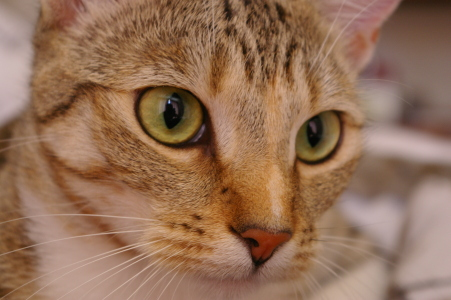
\includegraphics{figures/image_processed/chelsea.png}
    \caption{Chelsea without maxpooling}
    \label{fig:chelsea_original}
\end{figure}

\begin{figure}[]
    \centering
    
\includegraphics{figures/image_processed/chelsea_maxpooled.png}
    \caption{Chelsea with maxpooling}
    \label{fig:chelsea_maxpooled}
\end{figure}

\begin{figure}[]
    \centering
    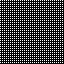
\includegraphics{figures/image_processed/checkerboard.png}
    \caption{Checkerboard without maxpooling}
    \label{fig:checkerboard_original}
\end{figure}

\begin{figure}[]
    \centering
    
\includegraphics{figures/image_processed/checkerboard_maxpooled.png}
    \caption{Checkerboard with maxpooling}
    \label{fig:checkerboard_maxpooled}
\end{figure}


\newpage
\subsubsection*{b)}
See \cref{fig:task2b} for the plot of the cross entropy loss for the test and training data. The final validation loss was calculated as $0.06696378275700904$, and the final validation accuracy was calculated as $0.9758$. We can notice overfitting when training loss is a lot smaller than validation loss. From \cref{fig:task2b}, we can notice that the test/validation loss is generally pretty similar to the training loss, and there doesn't seem to be enough information to conclude that the network has been overfitted. 

\begin{figure}[]
    \centering
    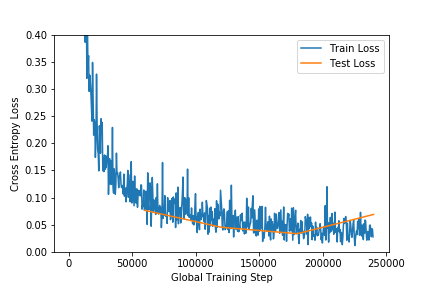
\includegraphics[width=1.00\textwidth]{figures/image_processed/task2_b.png}
    \caption{Cross entropy loss for training and test. 4 epochs}
    \label{fig:task2b}
\end{figure}

% Final Validation loss: 0.06696378275700904. Final Validation accuracy: 0.9758

\subsubsection*{c)}
See \cref{fig:task2c} for the plot of the cross entropy loss for the test and training data. The final validation loss was calculated as $0.021018466441450896$, and the final validation accuracy was calculated as $0.9932$. 

\begin{figure}[]
    \centering
    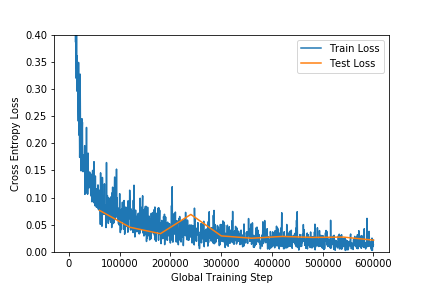
\includegraphics[width=1.00\textwidth]{figures/image_processed/task2_c.png}
    \caption{Cross entropy loss for training and test. 10 epochs}
    \label{fig:task2c}
\end{figure}

% Final Validation loss: 0.021018466441450896. Final Validation accuracy: 0.9932

\subsubsection*{d)}
See the result from \cref{fig:task2d}. 

\begin{figure}[]
    \centering
    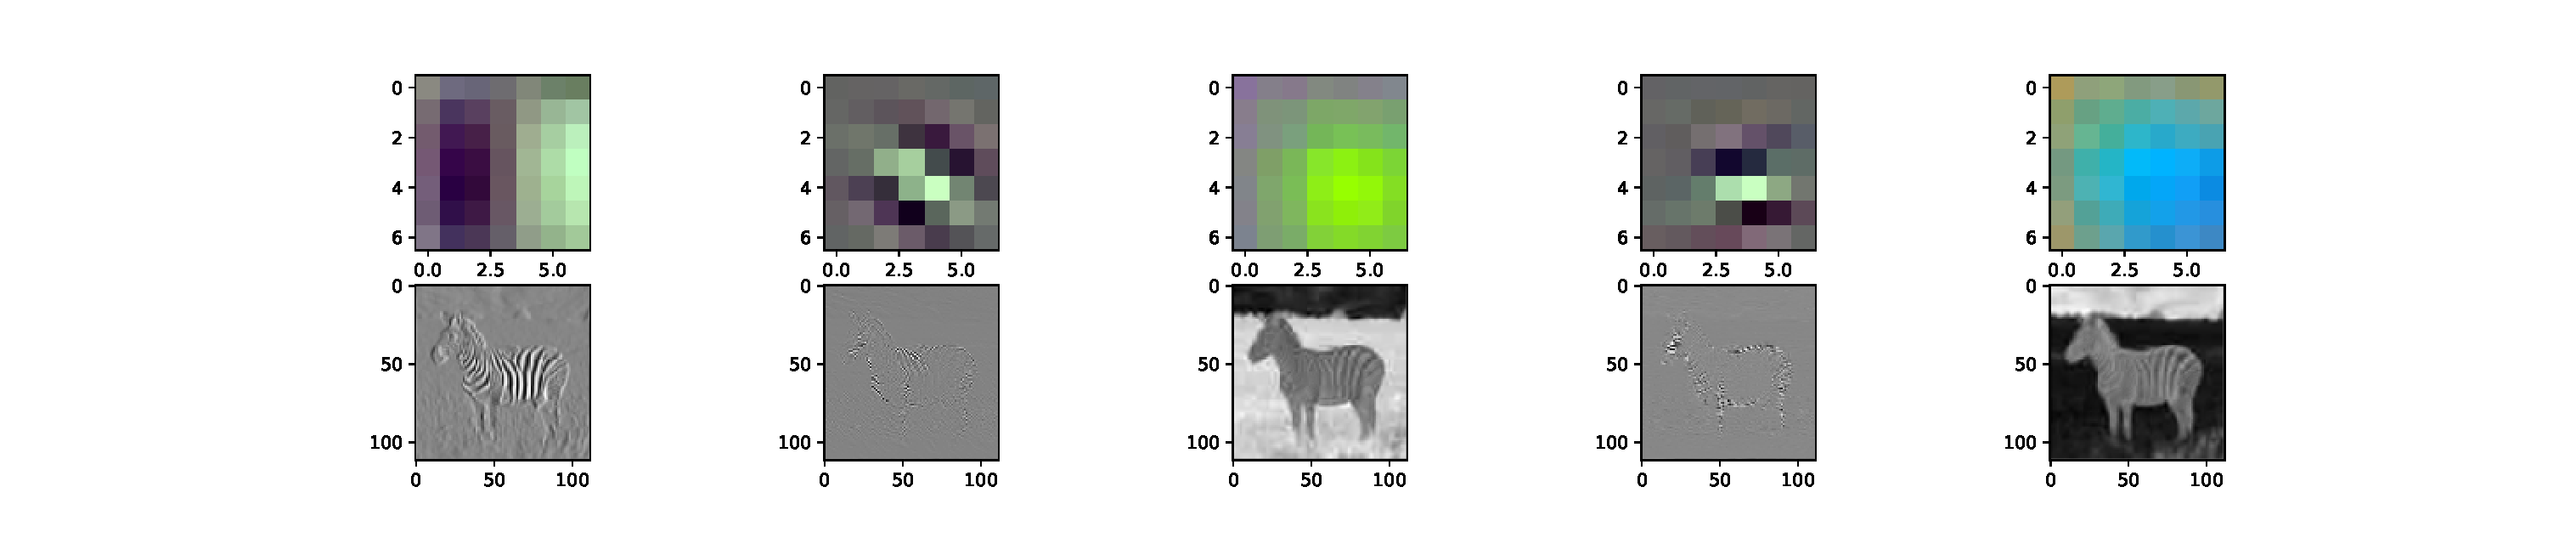
\includegraphics[width=1.00\textwidth]{figures/task2d_image.eps}
    \caption{Visualization of convolution layers with indices [5, 8, 19, 22, 34]}
    \label{fig:task2d}
\end{figure}

\subsubsection*{e)}
Kernel 5: 
This kernel is very similar to a Sobel x-kernel, with \textit{darker} weights on the left and \textit{lighter} weights on the right. Sobel x is used for edge detection/enhancement in the x-direction, and we can notice this in the image, as especially the stripes on the zebras stomach is highlighted, while the stripes on its face and neck are more diffuse, as these are more in the y-direction. 

The kernel seems to be more purple on the left, which indicates more red and blue, and more green/white on the right, which indicates more red, green and blue with a focus on green. What we may note, is that the focus seems to be on green, as the largest difference seems to be between these (no green on the left, mostly green on the right). 

Kernel 8: 
This kernel highlights the centre/diagonal, while the diagonal above and below are darker. This seems to emphasise the whiter diagonals of the image, but it also seems like this kernel is removing certain diagonals, as seen from the resulting image. 

Kernel 19: 
There is a huge focus on green in this kernel, with a focus on the bottom right of the kernel. So this kernel seems to extract the ground / grass. As yellow is a combination of green and red, we can see in the image that the grass is highlighted. 

Kernel 22: 
The kernel looks similar to a Sobel y-kernel, though it doesn't cover the entire kernel and more diagonalized.  This, then, seems to be detecting edges around larger objects. As we can see from the image, it seems to be detecting the edges (primarily in the y-direction) of the zebra. 

Kernel 34: 
This kernel is very similar to kernel 19, though with a focus on blue. From the image, we can see that the sky is highlighted, so this kernel seems to be extracting the sky, or other larger blue bodies (speculation: possibly water also?). 
